\documentclass[12pt,a4paper]{article}

\usepackage{float}
\restylefloat{figure}
\usepackage{hyperref}
\usepackage{graphicx}
\usepackage{gensymb}
\usepackage[title]{appendix}
\usepackage[dotinlabels]{titletoc}
\usepackage[nottoc,numbib]{tocbibind}
\usepackage{mathtools}
\usepackage[margin=0.5in]{geometry}
\renewcommand{\thefootnote}{\arabic{footnote}}

\newcommand*\wrapletters[1]{\wr@pletters#1\@nil}
\def\wr@pletters#1#2\@nil{#1\allowbreak\if&#2&\else\wr@pletters#2\@nil\fi}

\usepackage{enumitem}
\setenumerate{itemsep=0pt}

% Add support for multi-page tables.
\usepackage{longtable}

\pagenumbering{arabic}

\title{EE4DSA Coursework 2}
\author{Chris Cummins}

\begin{document}
\maketitle

\section{Disassembling the program ROM}

The file \texttt{extra/rom.asm} contains a heavily annotated
disassembled version of the safe unlocking program in a style inspired
by the AVR Assembler Syntax. The program tests for the safe code 4D5A.

The assembly code was generated automatically using a disassembler
developed for this purpose, available at
\url{http://chriscummins.cc/disassembler}. Based off of the
implementation of the first coursework disassembler, the functionality
has been extended to support the subroutine and interrupt
instructions, and development effort has been focused on making the
output easier to understand.

Generated label names now distinguish between subroutines, interrupt
handlers and sections, and the UI now supports syntax highlighting,
automatic comment generation, line highlighting and jumping to
sections (clicking on a branch or jump instruction will now take the
user to the specific address). Backwards compatibility with the first
coursework instruction set is ensured by allowing the user to select
between an initial program counter of either 0x00 or 0x08.

\begin{figure}[H]
  \centering
  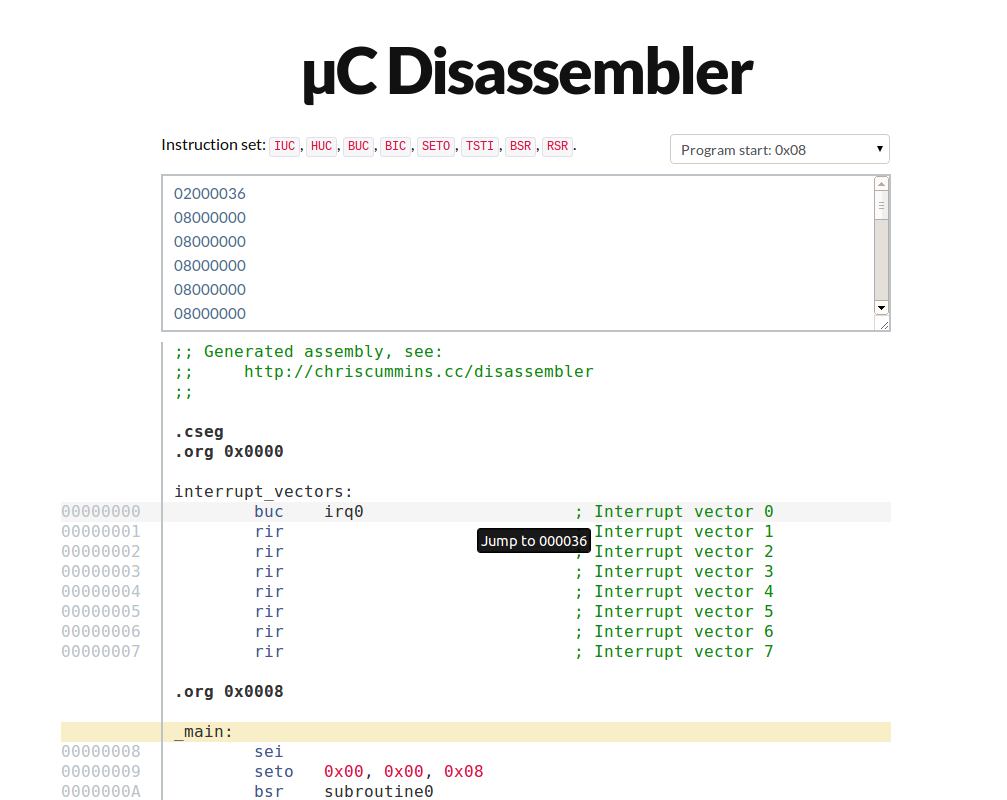
\includegraphics[width=6.4in]{assets/disassembler.png}
\end{figure}

The disassembler is implemented in 479 lines of JavaScript, with the
source code available at\\*
\url{http://chriscummins.cc/js/disassembler.js}.

\section{Modifying the ROM program}

The file \texttt{rom.dat} contains a modified ROM program which uses
the last four digits of my SUN number (5189) as the code to the
safe. The only modifications required were to the \texttt{AND}
components of the four \texttt{TSTI} instructions. The
\texttt{test\_bench\_inputs.dat} file was then modified so as to test
this new safe unlocking code.

\section{Implementing the Execution Unit}

The file \texttt{execution\_unit.vhd} contains my implementation of
the execution unit. Using three processes, the clocked logic updates
register states, while the immediate logic executes the specific
opcode. The program counter uses an input multiplexer to select the
source from between the stack, ROM, or counter enable/disabled.

The directory \texttt{reports/} contains a copy of the synthesis
reports. Note that there are unused bit warnings due to the fact that
we don't use all of the available in every register, for example the
status register, which only implements the test and interrupt flags.

\begin{verbatim}
$ make synthesis
Synthesis running...
WARNING:HDLCompiler:634 - "/home/chris/src/vhdl-exercises/ee4dsa/cw2/       \
  top_level.vhd" Line 88: Net <eu_intr[7]> does not have a driver.
WARNING:Xst:2935 - Signal 'eu_intr<7:1>', unconnected in block 'top_level', \
  is tied to its initial value (0000000).
WARNING:Xst:647 - Input <rom_data<23:17>> is never used. This port will be  \
  preserved and left unconnected if it belongs to a top-level block or it   \
  belongs to a sub-block and the hierarchy of this sub-block is preserved.
WARNING:Xst:647 - Input <ram_rdata<15:6>> is never used. This port will be  \
  preserved and left unconnected if it belongs to a top-level block or it   \
  belongs to a sub-block and the hierarchy of this sub-block is preserved.
WARNING:Xst:647 - Input <en> is never used. This port will be preserved and \
  left unconnected if it belongs to a top-level block or it belongs to a    \
  sub-block and the hierarchy of this sub-block is preserved.
WARNING:Xst:2404 -  FFs/Latches <current_sr<31:16>> (without init value)    \
  have a constant value of 0 in block <execution_unit>.
\end{verbatim}

Analysing the log \texttt{reports/xst.log} shows that the maximum
achievable frequency of the design is 170.837 MHz. The bottleneck in
this performance is the logic involved in the \texttt{next\_pc} input
multiplexer. The EU implementation could be refactored so as to remove
this third process, which would result in an increase to this maximum
achievable frequency; however, the benefit in readability and
abstraction that an explicit program counter multiplexer offers
outweighs the advantages of increase performance at this stage,
especially since we are well within the safe operating minimum of 125
MHz.

As we add further features in later courseworks such as the register
file and ALU, it may be necessary to refactor this logic into a two
process application. Other candidates for performance optimising
include the for loop used to set the interrupt handler address, and
removing some of the intermediate signals used to store register
data. This would reduce in shorter paths and fewer gate delays.

\newpage
\begin{verbatim}
Delay:               5.854ns (Levels of Logic = 5)
  Source:            reset_unit/cnt_6 (FF)
  Destination:       rom_unit/do_27 (FF)
  Source Clock:      clk rising
  Destination Clock: clk rising

  Data Path: reset_unit/cnt_6 to rom_unit/do_27
                                Gate     Net
    Cell:in->out      fanout   Delay   Delay  Logical Name (Net Name)
    ----------------------------------------  ------------
     FDE:C->Q              3   0.447   1.015  reset_unit/cnt_6 (reset_unit/cnt_6)
     LUT6:I0->O           11   0.203   0.883  rst_SW0 (N4)
     LUT6:I5->O            3   0.205   0.651  rst_1 (rst1)
     LUT5:I4->O            1   0.205   0.684  execution_unit/Mmux_next_pc6_SW3 (N36)
     LUT6:I4->O           18   0.203   1.050  execution_unit/Mmux_next_pc6 (eu_rom_addr<5>)
     LUT6:I5->O            1   0.205   0.000  rom_unit_Mram_addr[5]_GND_16_o_wide_mux_0_OUT41 (rom_unit/addr[5]_GND_16_o_wide_mux_0_OUT<4>)
     FDE:D                     0.102          rom_unit/do_4
    ----------------------------------------
    Total                      5.854ns (1.570ns logic, 4.284ns route)
                                       (26.8% logic, 73.2% route)
\end{verbatim}

\section{Testing the Execution Unit}

A video demonstration of the program can be found at
\url{http://youtu.be/VDQkSEcJUaA}, showing how the program behaves when
inputting a correct code, invalid code, and interrupting normal
program behaviour by resetting the board.

\end{document}
